\documentclass[10pt,a4j]{jarticle}
\usepackage[dvipdfmx]{graphicx}
\usepackage[dvipdfmx]{color}
\usepackage{url}
\usepackage{here}
\usepackage{amsmath}
\usepackage{subfig}

\newcommand{\figref}[1]{図\ref{#1}}
\newcommand{\subfigref}[2]{図\ref{#1}\subref{#2}}
\renewcommand{\eqref}[1]{式(\ref{#1})}



\renewcommand{\topfraction}{1.0}
\renewcommand{\bottomfraction}{1.0}
\renewcommand{\dbltopfraction}{1.0}
\renewcommand{\textfraction}{0.01}
\renewcommand{\floatpagefraction}{1.0}
\renewcommand{\dblfloatpagefraction}{1.0}
\setcounter{topnumber}{5}
\setcounter{bottomnumber}{5}
\setcounter{totalnumber}{10}

%----------表紙設定----------%
\makeatletter
\def\id#1{\def\@id{#1}}
\def\department#1{\def\@department{#1}}
\def\faculty#1{\def\@faculty{#1}}
\def\adviser#1{\def\@adviser{#1}}
\def\@maketitle{
\begin{center}
{\Large \@title \par} % 論文のタイトル部分
\vspace{40mm}
{\large \@date\par} % 提出年月日部分
\vspace{15mm}
{\large \@faculty \par} % 学部
\vspace{15mm}
{\large \@department \par} % 所属部分
\vspace{50mm}
{\large \@id \par} % 学籍番号
\vspace{5mm}
{\large \@author \par} % 氏名
\vspace{5mm}
{\large 指導教員:\ \@adviser \par} % 指導教員
\vspace{10mm}
{\large 豊橋技術科学大学 \par} %大学名
\end{center}
\par\vskip 1.5em
}
\makeatother

\date{\today} % 日付
\faculty{学部(工学)} % 学部
\department{情報・知能工学課程} % 所属課程
\id{153321} % 学籍番号
\author{加藤\ 翼} % 氏名
\adviser{三浦\ 純} % 指導教員

\begin{document}
%---表紙---%
%	\maketitle
%	\thispagestyle{empty}
%	\setcounter{page}{0}
%	\newpage
	
%---概要---%
\section{レンズの歪曲収差とは何か}
収差を大別すると、単色収差と色収差に分けられる。歪曲収差は単色収差のひとつである。
単色収差には記述方法の異なる光線収差と波面収差の分類があるが、物理的実体は同じであり、
光線収差を求めるために、屈折面においてスネルの法則を用いて光線を追跡するとき、近似していくなかで、光線収差には5つの分類が出来上がる。これはザイデルの5収差と呼ばれ、歪曲収差はそのひとつとされている。
歪曲収差は光軸に垂直な平面上にある物体は、光軸に垂直な平面上に結像するため、像は鮮明となる。しかし、光軸から離れた部分ほど形状が歪む性質が観測できる。歪む形には糸巻き型や樽型が挙げられる。
歪曲収差は像点のずれが像高の3乗に比例するため、像の大きさによって横倍率が異なることにより生じる。つまり、入射光線の画角または像高により、結像倍率が異なってしまう。

\begin{figure}[h]
	\centering
	\includegraphics[width=50mm]{image/dummy.png.eps}
	\caption{歪曲収差}
	\label{caption1}
\end{figure}

\begin{figure}[h]
    
    \centering
    \subfloat[糸巻き型]{\includegraphics[width=50mm]{image/dummy.png.eps} \label{shape1}}
    \subfloat[樽型]{\includegraphics[width=50mm]{image/dummy.png.eps} \label{shape2}}
    
    \caption{歪曲収差による観測できる形}
    \label{shape}
    \end{figure}\newpage
\section{レンズの歪曲収差の校正方法について}
歪曲収差は半径方向歪みに分類され、これはレンズの形状に起因する。
レンズの特性から、レンヌの中心から離れた場所を通過する光は近くを通過する光よりも大きく曲げられる。
この特性より、光学の中心において歪みは観測されなく、周辺部分に行くに従って歪みは大きくなる。
現実では、この歪みは小さいものであり、光学中心からみた半径を\begin{math}{r}\end{math}とし、\begin{math}{r=0}\end{math}付近でのテイラー級数を求め、近似値として表せる。
\begin{eqnarray}
  x_{corrected} & = & x(1+k_1 r^2+k_2 r^4+k_3 r^6) \\
  y_{corrected} & = & y(1+k_1 r^2+k_2 r^4+k_3 r^6)
\end{eqnarray}
一般的には、第二の項を用いるが、魚眼カメラのように歪みの大きいカメラの場合は第三の項を使って近似する。

____________________________________________

この他にも、レンズの組み合わせによる校正方法が挙げられる。
\newpage
\section{歪曲収差以外の収差とその特徴について}
1章にて、収差には単色収差と色収差が存在すると述べた。また、単色収差にはザイデルの5収差がある。
\subsection{ザイデルの5収差}
\subsubsection{球面収差}
球面収差とは、レンズ面が球面であることにより発生する収差である。ここで、\eqref{seidelx},\eqref{seidely}から球面収差の項のみを考える。つまり、
\begin{eqnarray}
	\Delta x' & = & A r^3 \sin \theta \\
	\Delta y' & = & A r^3 \cos \theta
\end{eqnarray}
以上の式より、球面収差は入射高の3乗に比例し、像の高さに依存しない。口径を絞り込むことによって収差は少なくなるといえる。
%球面収差とは、光軸から離れた光線ほど、光学系浸透後に、軸上での像点が手前にできてしまうことをいう。他の収差と異なり、像面全体に同量の収差を生じさせる。また光軸上の物体に対しても収差が存在するのは、球面収差だけとなってである。
\begin{figure}[h]
	\centering
	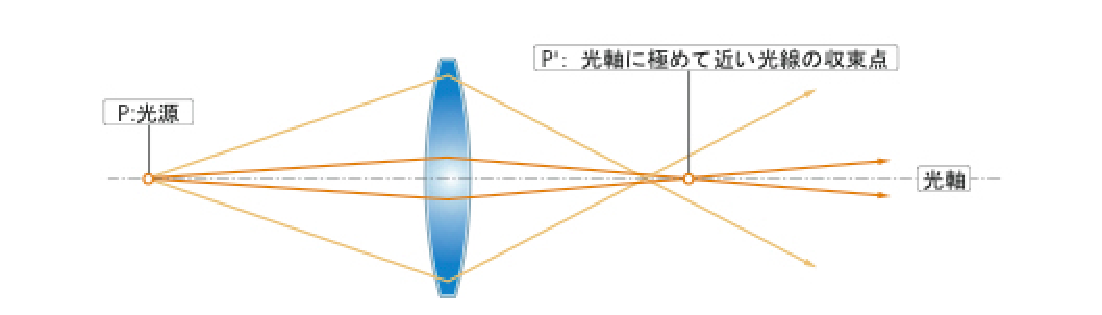
\includegraphics[height=30mm]{image/kyumen.png.eps}
	\caption{球面収差\ \cite{cite1}}
	\label{caption1}
\end{figure}
\subsubsection{コマ収差}
コマ収差とは、光軸より離れた物点の横倍率が物点の位置により異なる収差のことをいう。ここで、\eqref{seidelx},\eqref{seidely}からコマ収差の項のみを考える。つまり、
\begin{eqnarray}
	\Delta x' & = & B r^2 y\sin 2 \theta \\
	\Delta y' & = & B r^2 y (2+\cos 2\theta)
\end{eqnarray}
以上の式より、コマ収差は入射高の2乗に比例し、像高に比例する。つまり、口径を絞り込むことによって収差は少なくなるといえる。
\begin{figure}[h]
	\centering
	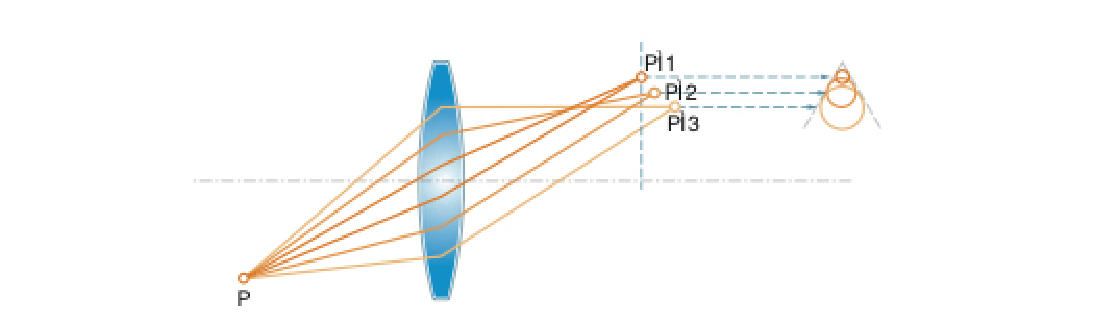
\includegraphics[height=30mm]{image/koma.png.eps}
	\caption{コマ収差\ \cite{cite1}}
	\label{caption1}
\end{figure}
\vspace{10cm}
\subsubsection{非点収差と像面収差}
非点収差とは、子午光線と球欠光線に対する焦点距離の違いのことをいう。
像面収差とは、光軸に平行な光線と傾いた光線が、光軸に垂直な同一面に結像しないことをいう。
ここで、非点収差と像面収差の項を考える。したがって、
\begin{eqnarray}
	\label{seidelx}
	\Delta x' & = & D r y^2 \sin \theta \\
	\label{seidely}
	\Delta y' & = & (2C+D)r y^2 \cos \theta 
\end{eqnarray}
以上の式から、どちらの収差も、入射高に比例し、像高の2乗する。また、
像面収差は非点収差と異なり、湾曲も起こる。
\begin{figure}[h]
	\centering
	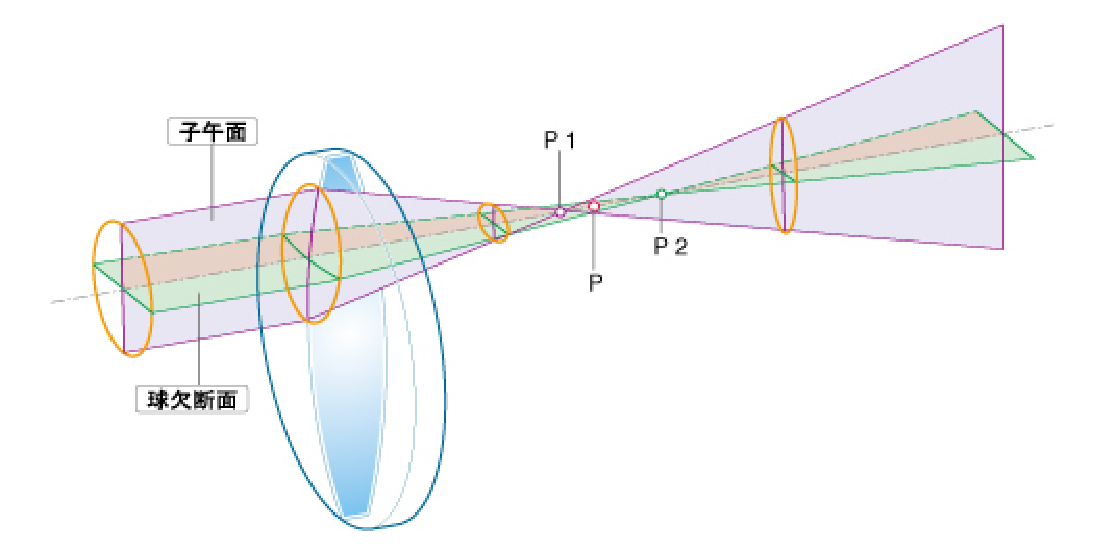
\includegraphics[height=40mm]{image/hiten.png.eps}
	\caption{非点収差\ \cite{cite1}}
	\label{caption1}
\end{figure}
\begin{figure}[h]
	\centering
	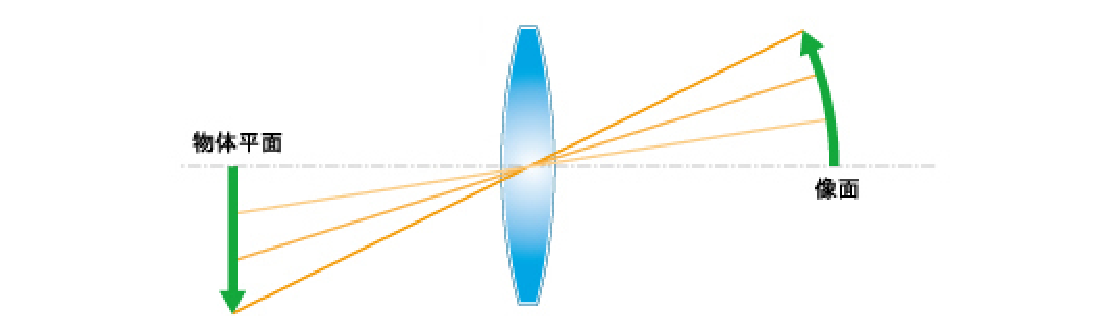
\includegraphics[height=30mm]{image/zomen.png.eps}
	\caption{像面収差\ \cite{cite1}}
	\label{caption1}
\end{figure}

\subsection{色収差}
\subsubsection{軸上色収差}
軸上色収差とは、光の波長によって光軸上で結像位置が異なる収差のことをいう。凸レンズと凹レンズを組み合わせることによって防ぐことができる。
\begin{figure}[h]
	\centering
	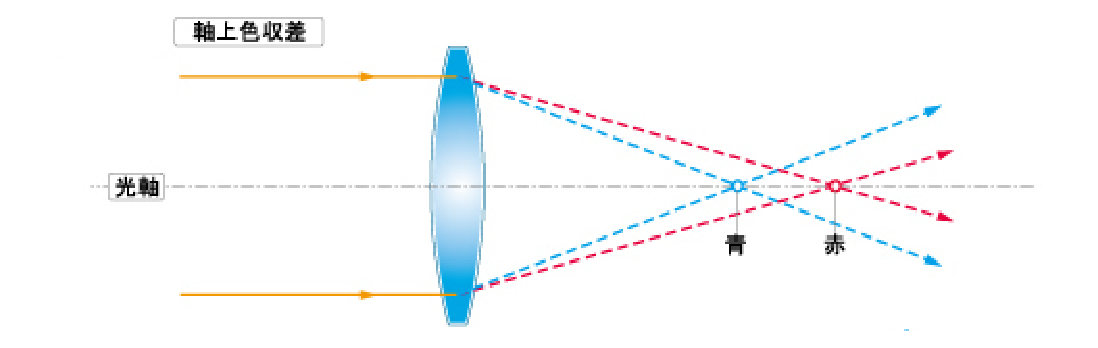
\includegraphics[height=30mm]{image/jikujo.png.eps}
	\caption{軸上色収差\ \cite{cite1}}
	\label{caption1}
\end{figure}
\subsubsection{倍率色収差}
倍率色収差とは、光の波長によって像の大きさが異なる収差のことをいう。この像の大きさの違いは波長による屈折率が異なることによって生じる。波長の像倍率の補正を行うことによって収差を防ぐことができる。
\begin{figure}[h]
	\centering
	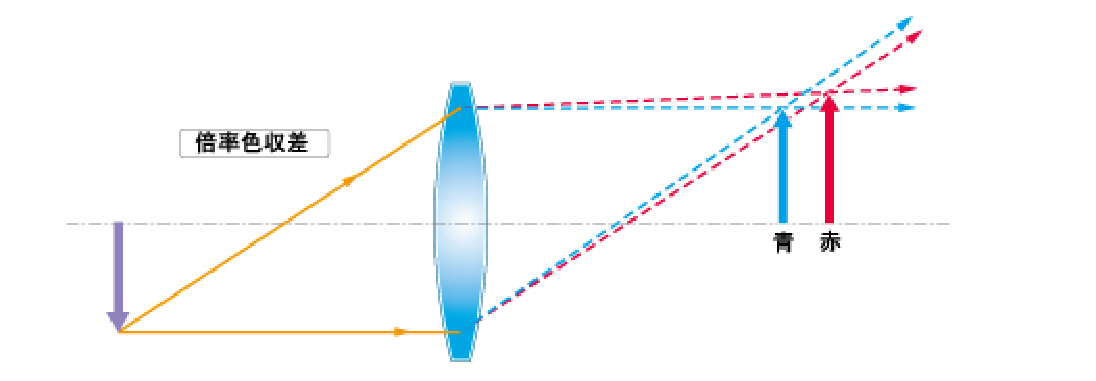
\includegraphics[height=30mm]{image/bairitsu.png.eps}
	\caption{倍率色収差\ \cite{cite1}}
	\label{caption1}
\end{figure}
\begin{thebibliography}{9}
	\fontsize{8.5pt}{0pt}\selectfont
	\bibitem{bunken1}{M.ボウン,E.ウォルフ,(訳:草川徹・横田英嗣),"\ 光学の原理I\ ",1994年第八版}
	\bibitem{bunken2}{Mejiro Genossen,"\ 光学設計の基礎知識\ "}
	\bibitem{bunken3}{左貝潤一,"\ 光学機器の知識\ ",2013年第一版}
	\bibitem{cite1}{ニコン,"双顕微鏡の構造と光学技術",\url{http://www.nikonvision.co.jp/how_to/guide/binoculars/technologies/technologies_08.htm}}
\end{thebibliography}	


\end{document}